% ==============================================================================
% Fichier : 06_sujets_connexes.tex
% Description : Discussions sur des Sujets Connexes (IA, Fraude)
% ==============================================================================

\chapter{Sujets Connexes : IA et Fraude dans les SI}\label{chap:07_sujets_connexes}

Au-delà des processus classiques, l'auditeur moderne doit adresser des défis technologiques et comportementaux nouveaux. Ce chapitre traite de l'impact de l'Intelligence Artificielle et de la fraude assistée par les systèmes d'information.

\section{L'Intelligence Artificielle et l'Audit}
% ------------------------------------------------------------------------------

L'IA est à la fois un sujet d'audit (l'entreprise utilise-t-elle l'IA correctement ?) et un outil pour l'auditeur (l'IA peut-elle m'aider à auditer ?).

\subsection{Le Rôle et l'Impact de l'IA dans les SI}

Les entreprises comme \textbf{Lizbiz's} intègrent l'IA pour optimiser leurs processus :
\begin{itemize}
    \item \textbf{Automatisation :} Traitement des commandes, chatbots service client.
    \item \textbf{Prédictif :} Anticipation des stocks, analyse des risques financiers.
\end{itemize}

\subsection{Les Risques Liés à l'IA}

L'auditeur doit identifier les risques spécifiques à ces nouvelles technologies :

\begin{table}[h!]
\centering
\begin{tabular}{p{4cm}p{8cm}}
    \toprule
    \textbf{Type de Risque} & \textbf{Description} \\
    \midrule
    \textbf{Biais Algorithmiques} & L'IA prend des décisions discriminatoires basées sur des données biaisées (ex: refus de crédit injustifié). \\
    \textbf{Boîte Noire (Black Box)} & Impossibilité d'expliquer comment l'IA a pris une décision (manque de traçabilité). \\
    \textbf{Sécurité des Données} & L'IA a besoin de masses de données (Big Data), augmentant le risque de fuite. \\
    \textbf{Dépendance} & L'entreprise perd le contrôle humain sur des processus critiques. \\
    \bottomrule
\end{tabular}
\end{table}

\subsection{Enjeux pour l'Auditeur}

Face à l'IA, l'auditeur doit adapter sa démarche :
\begin{enumerate}
    \item \textbf{Auditer l'Algorithme :} Vérifier la qualité des données d'entrée (Garbage In, Garbage Out) et la pertinence du modèle.
    \item \textbf{Vérifier l'Éthique :} S'assurer que les décisions de l'IA respectent la loi (RGPD) et l'éthique de l'entreprise.
    \item \textbf{Utiliser l'IA :} L'auditeur peut utiliser des outils d'IA pour analyser des volumes de données impossibles à traiter manuellement (détection d'anomalies automatiques).
\end{enumerate}

\begin{boxlizbiz}
\textbf{Cas Lizbiz's :}
L'entreprise utilise une IA pour gérer les stocks. L'auditeur constate que l'IA commande des stocks énormes pour des produits peu vendus. Analyse : Les données historiques utilisées pour "entraîner" l'IA contenaient des erreurs de saisie de l'année précédente. \textbf{Recommandation :} Nettoyer les données d'entraînement et mettre en place un contrôle humain avant validation des commandes fournisseurs.
\end{boxlizbiz}

% ------------------------------------------------------------------------------
\section{La Fraude dans et par les Systèmes d'Information}
% ------------------------------------------------------------------------------

Le SI est un terrain fertile pour la fraude : il centralise l'argent, les actifs et les données, tout en offrant une certaine anonymat technique.

\subsection{Nature de la Fraude Informatique}

La fraude peut prendre plusieurs formes :
\begin{itemize}
    \item \textbf{Fraude Interne :} Complaisance, détournement de fonds, vol de données par un employé.
    \item \textbf{Fraude Externe :} Hameçonnage (Phishing), escroquerie au président, piratage.
    \item \textbf{Fraude aux Données :} Falsification des états financiers via le système comptable.
\end{itemize}

\subsection{L'Impact de la Fraude}

Les conséquences vont au-delà de la perte financière directe :
\begin{itemize}
    \item \textbf{Perte d'Image :} Difficile à quantifier mais destructrice (perte de confiance clients).
    \item \textbf{Perte de Compétitivité :} Vol de secrets industriels ou de clientèle.
    \item \textbf{Coût de Remédiation :} Frais juridiques, amendes, reconstruction du SI.
\end{itemize}

\subsection{Les Parades (Dispositifs Anti-Fraude)}

L'auditeur vérifie l'existence et l'efficacité des dispositifs de prévention :

\subsubsection{Contrôles Préventifs}
\begin{itemize}
    \item Séparation des tâches (la personne qui commande n'est pas celle qui paie).
    \item Gestion stricte des habilitations (Principe du moindre privilège).
    \item Sensibilisation des employés au Phishing.
\end{itemize}

\subsubsection{Contrôles Détectifs}
\begin{itemize}
    \item Revue des logs et traces d'activité.
    \item Analyse de données (Data Mining) pour repérer des anomalies (ex: factures avec des montants ronds, doubles paiements).
    \item Ligne éthique (Whistleblowing) pour signaler les comportements suspects.
\end{itemize}

\begin{boxlizbiz}
\textbf{Cas Lizbiz's :}
Une rumeur de fraude circule sur la création de "Fournisseurs Fictifs".
\textbf{Mission de l'Auditeur :} Utiliser des requêtes SQL sur la base de données fournisseurs pour identifier des anomalies :
\begin{itemize}
    \item Fournisseurs créés récemment avec des montants énormes.
    \item Adresse du fournisseur identique à l'adresse d'un employé.
    \item Numéro de compte bancaire IBAN suspect.
\end{itemize}
L'analyse de données permet de détecter la fraude bien plus vite qu'un audit manuel papier.
\end{boxlizbiz}
% ------------------------------------------------------------------------------
\subsection{Le Cadre Réglementaire : L'IA Act et la Classification des Risques}
% ------------------------------------------------------------------------------

L'auditeur doit évaluer les systèmes d'IA de l'entreprise (comme les outils de prédiction de stocks de \textbf{LiZbiZ}) au regard des nouvelles réglementations internationales. L'approche est basée sur le niveau de risque :

\begin{description}
    \item[Risque Inacceptable :] Systèmes interdits (ex: notation sociale, surveillance biométrique en temps réel).
    \item[Haut Risque :] Systèmes impactant la sécurité ou les droits fondamentaux (ex: recrutement automatisé, gestion des infrastructures critiques). \textit{Audit obligatoire}.
    \item[Risque Limité :] Obligations de transparence (ex: Chatbots, Deepfakes). L'utilisateur doit savoir qu'il interagit avec une IA.
    \item[Risque Minime :] Aucune obligation particulière (ex: filtres anti-spam).
\end{description}
% ------------------------------------------------------------------------------
\section{L'Audit Forensics : De la Constatation à la Preuve Judiciaire}
% ------------------------------------------------------------------------------

Lorsque l'auditeur identifie une fraude, la mission bascule dans une phase d'investigation numérique (\textit{Digital Forensics}). L'objectif n'est plus seulement l'amélioration, mais la manifestation de la vérité.

\subsection{La Chaîne de Garde (Chain of Custody)}
Pour qu'une preuve soit admissible, l'auditeur doit documenter de manière ininterrompue qui a manipulé l'élément de preuve, où et quand.

\subsection{Principes de Saisie de Preuve Numérique}
L'auditeur doit suivre une méthodologie stricte pour ne pas polluer les traces :
\begin{enumerate}
    \item \textbf{Collecte de la volatilité :} Capturer la mémoire vive (RAM) avant d'éteindre la machine (car elle contient les clés de chiffrement et connexions actives).
    \item \textbf{Duplication bit-à-bit :} Utilisation de bloqueurs d'écriture matériels pour créer une image miroir des supports (Disques durs, clés USB).
    \item \textbf{Calcul d'empreinte (Hash) :} Utilisation d'algorithmes (SHA-256) pour garantir l'intégrité de la copie.
\end{enumerate}

\begin{boxalert}
\textbf{Conseil de l'Expert :} Ne travaillez jamais sur l'original. Toute analyse doit être effectuée sur une copie certifiée conforme.
\end{boxalert}

% ------------------------------------------------------------------------------
\subsection{Schématisation : Le Triangle de la Fraude}
% ------------------------------------------------------------------------------

L'auditeur doit comprendre les trois facteurs qui poussent un individu (par exemple un employé de \textbf{LiZbiZ}) à passer à l'acte.

\begin{center}
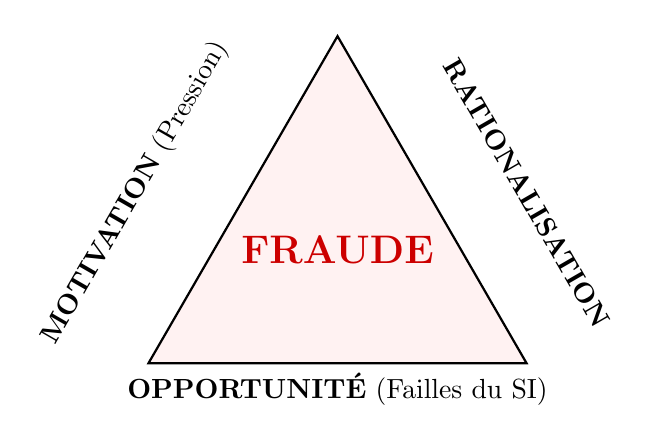
\begin{tikzpicture}[scale=1.2]
    \coordinate (A) at (0,0);
    \coordinate (B) at (4,0);
    \coordinate (C) at (2,3.46);
    
    \draw[thick, fill=red!5] (A) -- (B) -- (C) -- cycle;
    
    \node[below] at (2,0) {\textbf{OPPORTUNITÉ} (Failles du SI)};
    \node[left] at (1,1.8) {\rotatebox{60}{\textbf{MOTIVATION} (Pression)}};
    \node[right] at (3,1.8) {\rotatebox{-60}{\textbf{RATIONALISATION}}};
    
    \node at (2,1.2) {\textcolor{red!80!black}{\Large \textbf{FRAUDE}}};
\end{tikzpicture}
\end{center}
